\section{Results}
\label{sec:results}

	% Methodology
	To assess the costs of creating and waiting for a task, we created
	a synthetic benchmark that write each byte of 16 memory pages, e.g., 64~KB.
	To guarantee 95\% confidence, 50 replications were performed, the first 10
	being discarded to ignore the warm-up period.

	\begin{table}[t]
	\centering
	\caption{Benchmark parameters for experiments.}
	\label{tab:parameters}
	\begin{tabular}{lccc}
	\toprule
			\textbf{Benchmark}   & \textbf{\#Tasks} & \textbf{\#Threads} & \textbf{Memory} \\
			\midrule
			Single Dispatcher    & 1 to 29          & 1                  & 8~KB            \\
			Multiple Dispatchers & 1 to 29          & 14                 & 112~KB          \\
			Threads              & 1 to 29          & 1 to 29            & [8, 232]~KB     \\
			\bottomrule
	\end{tabular}
	\end{table}

	Table~\ref{tab:parameters} shows the application of this benchmark replicated in three
	different scenarios:
	\begin{enumerate*}[label=(\roman*)]
		\item A single dispatcher handle all tasks sequentially;
		\item Each free slave core contains a different dispatcher serving
			tasks in parallel, resulting in 14 dispatchers;
		\item One thread for each task, ranging from 1 to 29 threads.
	\end{enumerate*}
	The number of tasks was limited to the possible number of simultaneous
	threads within the microkernel not replicate the behavior of tasks in user
	threads. The amount of tasks and threads involved defines into the amount
	of memory required to execute each scenario, where each thread uses 8~KB
	for the stacks. Based on this, we can discern that much no extra effort,
	the user can use task abstraction with dispatchers and keep the amount of
	memory used controlled.

	% Time
	Figure~\ref{fig:time} shows the execution time in $\mu$s for each scenario.
	The times collected are made up of the dispatch/create and wait/join period
	of a task/thread.  Comparing the execution of a single task, the use of
	only one dispatcher showed superior performance to the other scenarios
	because there is no competition for the consumption of tasks, exploring the
	location of the data, and do not require the cost of the creation of a new
	thread. Between	7 to 13 tasks, all scenarios behaved similarly performance
	because the overhead of thread creation and concurrency were balanced by
	the workload of the single dispatcher. After 14 tasks, it is possible to
	notice an increase in the scenario of threads because from that moment,
	there are more threads than cores and they start to compete for execution
	time. In contrast, the scenario with 14 dispatchers showed a lower
	execution time because it needs less time to dispatch and consume a task
	than to create a thread. The single dispatcher scenario has steadily
	increased because the tasks are of regular size. Considering that the tasks
	are of regular size, share memory pages, and are executed in dedicated
	cores, the proposed mechanism showed performance similar to the scenario
	that uses specific threads per task.

	\begin{figure}[t]
			\centering
			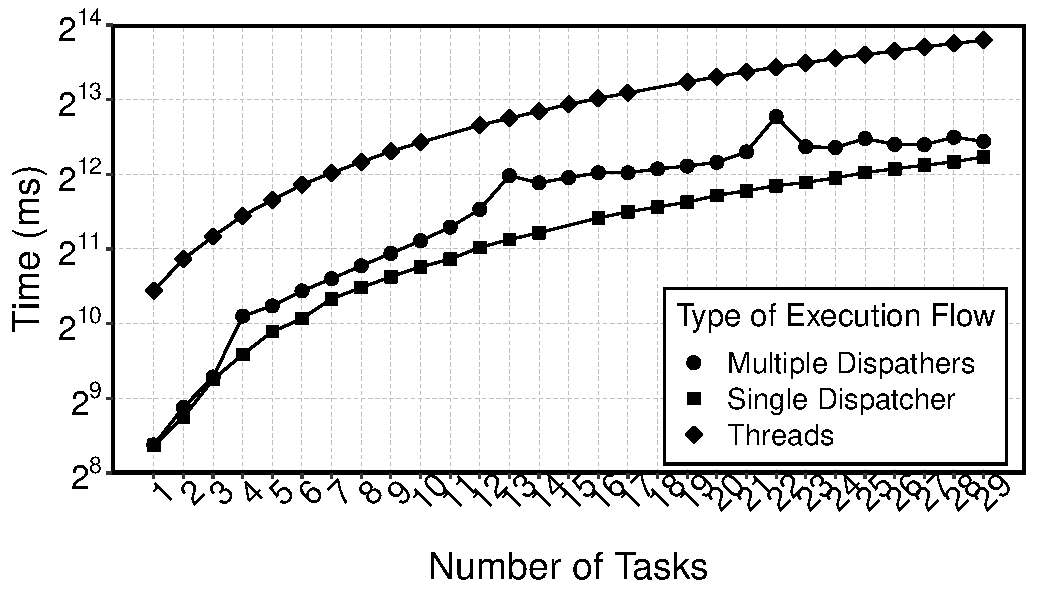
\includegraphics[width=0.97\linewidth]{tasks-time}
			\caption{Runtime Results.}
			\label{fig:time}
	\end{figure}
